\documentclass[a4paper,12pt]{report}
\usepackage[utf8]{inputenc}
\usepackage[T1]{fontenc}
\usepackage[french]{babel}
\usepackage{graphicx}
\usepackage{geometry}
\usepackage{fancyhdr}
\usepackage{hyperref}
\usepackage{float}
\usepackage{titlesec}
\usepackage{xcolor}

% Configuration des marges
\geometry{hmargin=2.5cm,vmargin=2.5cm}

% Configuration des en-têtes et pieds de page
\pagestyle{fancy}
\fancyhf{}
\lhead{\textbf{INE3 : Communication P2P}}
\rhead{Rapport de TP1}
\cfoot{\thepage}

% Configuration des liens hypertextes
\hypersetup{
    colorlinks=true,
    linkcolor=black,
    filecolor=magenta,      
    urlcolor=blue,
}

\begin{document}

%===========================================================
% PAGE DE GARDE
%===========================================================
\begin{titlepage}
    \centering
    \vspace*{1cm}
    
    \includegraphics[width=0.4\textwidth]{imgs/logo_inpt.png} % Remplacez par le logo de l'INPT si vous l'avez, sinon commentez cette ligne
    
    \vspace{2cm}
    
    {\Large \textbf{Institut National des Postes et Télécommunications}}\\[1.5cm]
    
    {\Large \textbf{Module : Communication P2P en temps réel sur le web (INE3)}}\\[0.5cm]
    {\huge \textbf{Rapport de TP1 : Les Servlets HTTP}}\\[0.5cm]
    {\large \textit{Implémentation via Python Flask : Une approche moderne des concepts JEE}}\\[2cm]
    
    \textbf{Réalisé par :}\\
    Aymane ASKRI\\[2cm]
    
    \textbf{Encadré par :}\\
    Asmae ELHAMZAOUI\\[2cm]
    
    \vfill
    
    {\large Année Universitaire : 2025-2026}
    
\end{titlepage}

%===========================================================
% TABLE DES MATIÈRES
%===========================================================
\tableofcontents
\newpage

%===========================================================
% INTRODUCTION
%===========================================================
\chapter*{Introduction}
\addcontentsline{toc}{chapter}{Introduction}

L'objectif initial de ce TP est de manipuler le protocole HTTP en utilisant la plateforme JEE et sa composante Servlet. Cependant, afin de se concentrer sur la maîtrise des concepts architecturaux (MVC, cycle de vie HTTP, Statelessness) plutôt que sur la complexité de configuration de Java, ce travail pratique a été réalisé en utilisant le langage \textbf{Python} et le micro-framework \textbf{Flask}.

Cette approche permet de reproduire fidèlement l'architecture demandée tout en offrant un code plus concis et lisible. Ce rapport détaille les étapes de réalisation et les extensions demandées, en mettant en parallèle les concepts Java EE et leur implémentation Python.

\chapter{Réalisation des Extensions}

%===========================================================
% EXTENSION 1
%===========================================================
\section{Intégration d’une Base de Données SQLite dans l’Application Flask}

Pour cette extension, nous avons remplacé la technologie JDBC (Java Database Connectivity) par le module \texttt{sqlite3} natif de Python. SQLite a été choisi pour sa légèreté, évitant l'installation d'un serveur lourd comme MySQL pour un environnement de TP, tout en respectant la logique SQL standard.

\subsection*{Le Formulaire HTML}
Voici le code du formulaire permettant la saisie de l'utilisateur :

\begin{figure}[H]
    \centering
    \includegraphics[width=0.9\textwidth]{imgs/form.png}
    \caption{Code du formulaire HTML}
\end{figure}

\subsection*{Le Contrôleur (App.py)}
Ce fichier remplace la classe \texttt{GreetingServlet} ainsi que la configuration \texttt{web.xml}. Il gère le routage et la logique métier.

\begin{figure}[H]
    \centering
    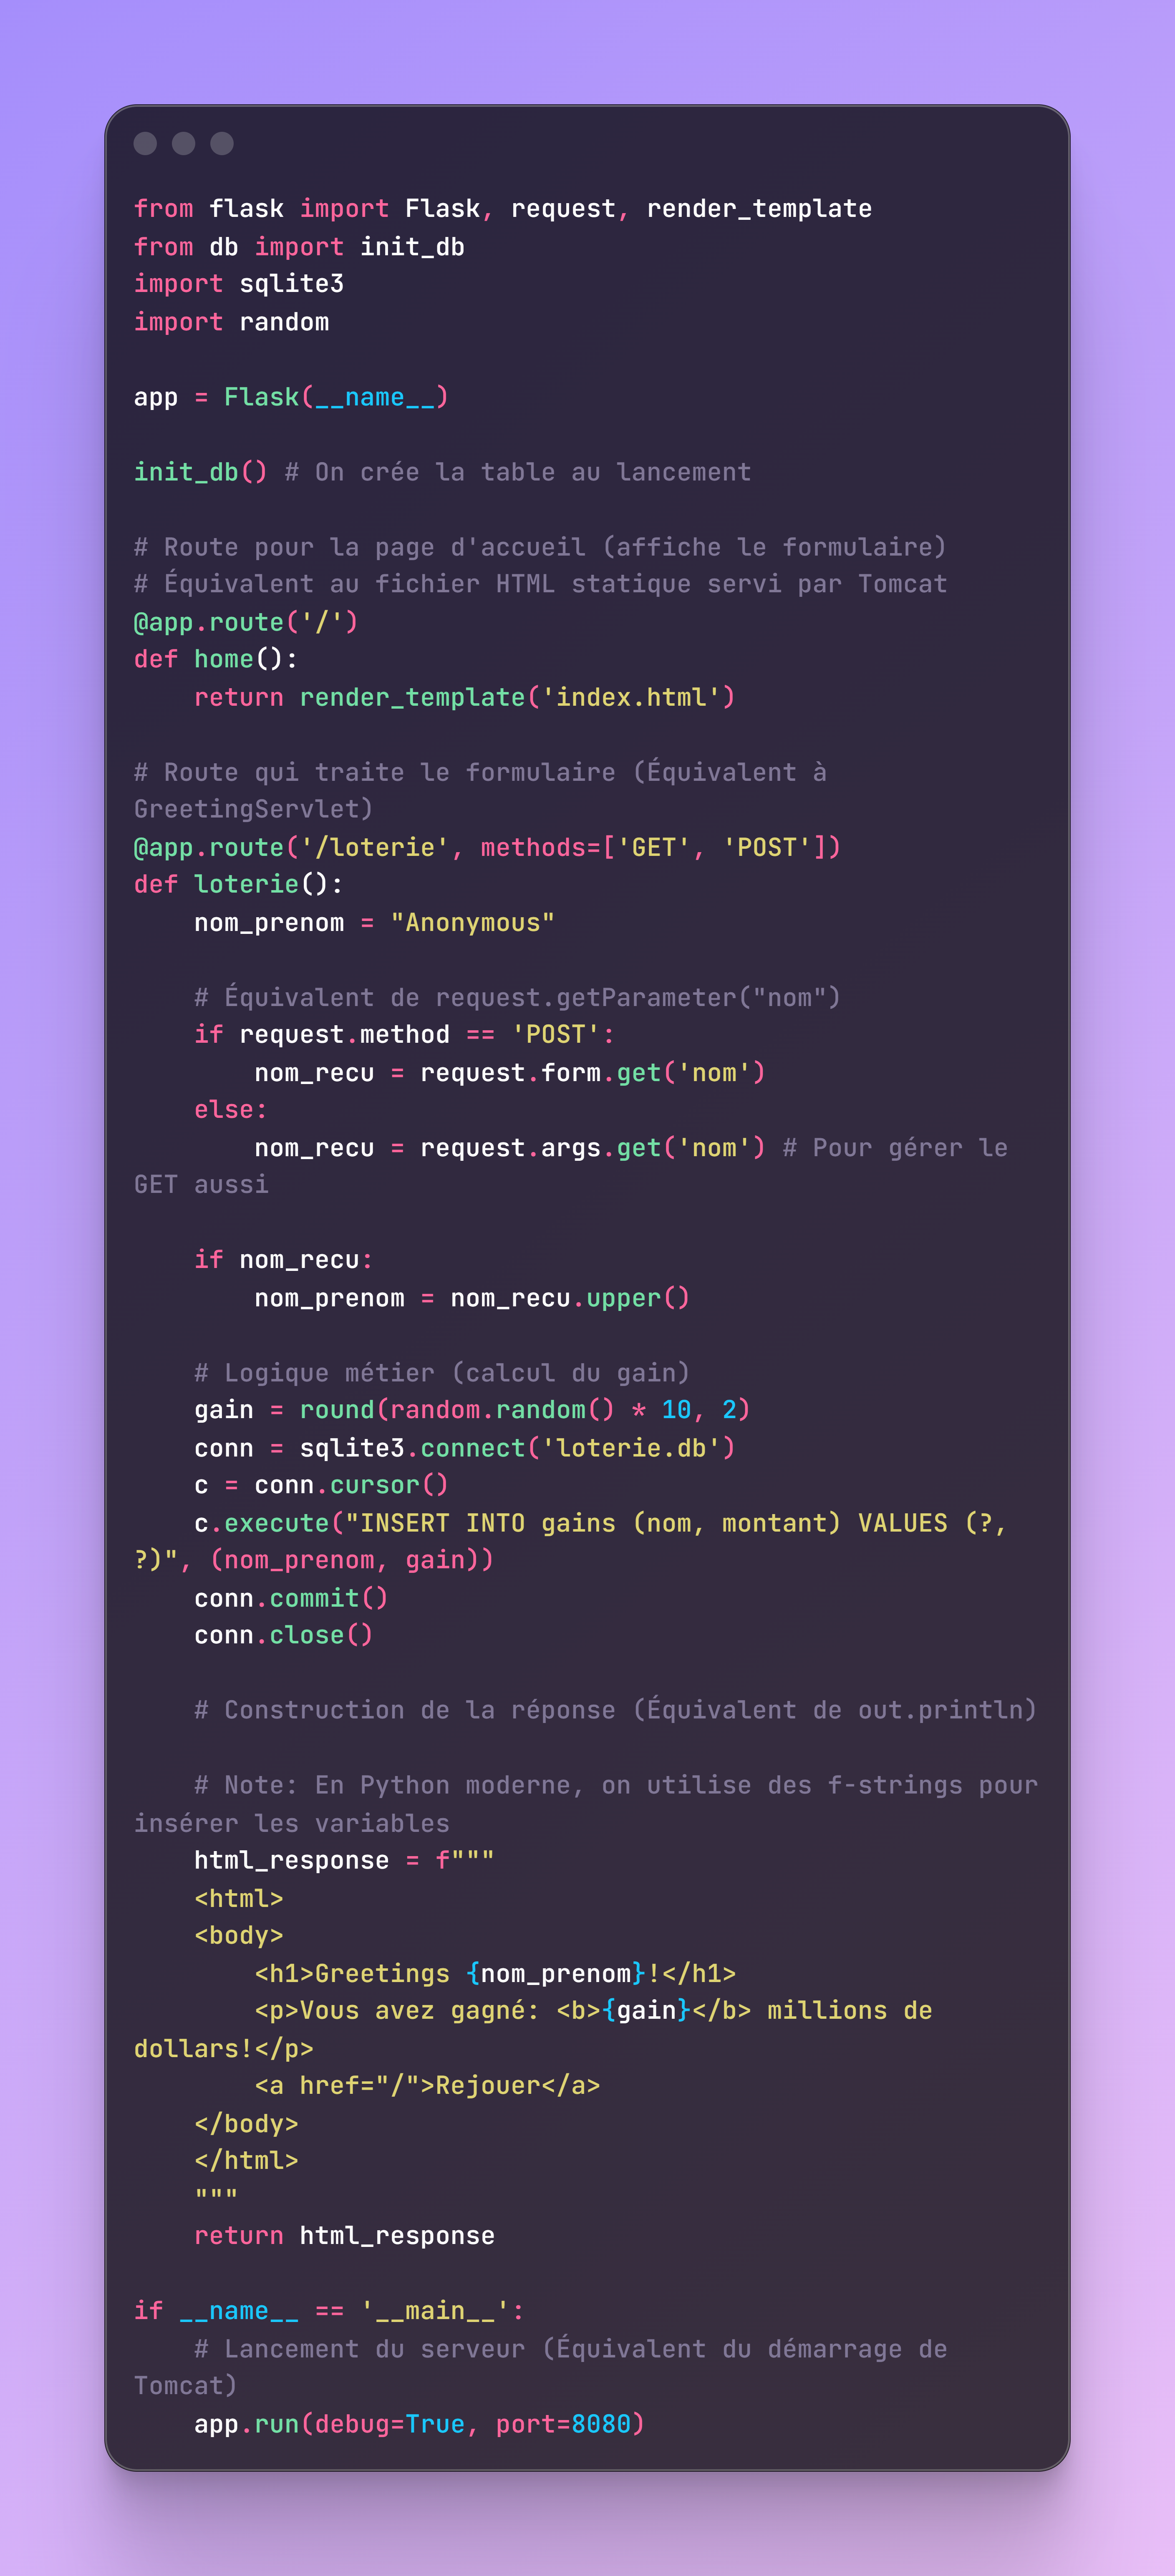
\includegraphics[width=0.9\textwidth]{imgs/code1.png}
    \caption{Code principal de l'application Flask (app.py)}
\end{figure}

\subsection*{La Couche de Données (DB.py)}
Python intègre SQLite par défaut. Ce module gère la persistance des données (gains de loterie).

\begin{figure}[H]
    \centering
    \includegraphics[width=0.9\textwidth]{imgs/code2.png}
    \caption{Gestion de la base de données (db.py)}
\end{figure}

\newpage

%===========================================================
% EXTENSION 2
%===========================================================
\section{Mise en Place d’un Système de Rôles et de Restrictions d’Accès}

Pour restreindre l'accès, nous utilisons le concept de \textbf{Décorateur} en Python. C'est l'équivalent fonctionnel des mécanismes de sécurité basés sur les rôles dans le conteneur de servlets.

Voici comment créer un décorateur pour bloquer les utilisateurs ne possédant pas le rôle 'tomcat' :

\begin{figure}[H]
    \centering
    \includegraphics[width=0.9\textwidth]{imgs/code3.png}
    \caption{Décorateur pour la vérification du rôle utilisateur}
\end{figure}

%===========================================================
% EXTENSION 3
%===========================================================
\section{Sécurité et Blacklist (Filtres)}

En Java EE, on utilise des \texttt{Filters} pour intercepter les requêtes. En Python Flask, on utilise également des \textbf{Décorateurs} pour appliquer une logique transversale (AOP - Aspect Oriented Programming).

Voici l'implémentation d'un décorateur pour bloquer une liste noire (Blacklist) d'utilisateurs :

\begin{figure}[H]
    \centering
    \includegraphics[width=0.9\textwidth]{imgs/code4.png}
    \caption{Implémentation du filtre Blacklist via un décorateur}
\end{figure}

\newpage

%===========================================================
% EXTENSION 4
%===========================================================
\section{Utiliser JSP (Templates)}

L'instruction demande de ne plus écrire le code HTML à l'intérieur du code métier (Java/Python). Flask utilise le moteur de template \textbf{Jinja2}, qui est l'équivalent direct de la technologie \textbf{JSP} (JavaServer Pages).

\subsection*{Le Template (Vue)}
Nous créons un fichier \texttt{templates/resultat.html} qui contient la structure de la page avec des placeholders pour les variables dynamiques.

\begin{figure}[H]
    \centering
    \includegraphics[width=0.9\textwidth]{imgs/code5.png}
    \caption{Fichier Template Jinja2 (resultat.html)}
\end{figure}

\subsection*{Modification du Contrôleur}
Nous modifions la fonction Python pour utiliser la méthode \texttt{render\_template}, séparant ainsi la vue du contrôleur.

\begin{figure}[H]
    \centering
    \includegraphics[width=0.9\textwidth]{imgs/code6.png}
    \caption{Appel du moteur de template dans le contrôleur}
\end{figure}

%===========================================================
% EXTENSION 6
%===========================================================
\section{Gestion des erreurs (404, 500)}

Cette partie correspond à la configuration de la balise \texttt{<error-page>} dans le fichier \texttt{web.xml} de Java EE. En Flask, nous utilisons des gestionnaires d'erreurs (\texttt{errorhandler}) spécifiques.

\begin{figure}[H]
    \centering
    \includegraphics[width=0.9\textwidth]{imgs/code7.png}
    \caption{Gestion personnalisée des codes d'erreur HTTP}
\end{figure}

\chapter{Synthèse des Concepts : Architecture Web et Protocole HTTP}

Ce Travail Pratique (TP) a permis d'explorer les fondements du développement web dynamique et la mise en œuvre du protocole HTTP au sein d'une architecture client-serveur. Bien que l'implémentation ait été réalisée avec le framework Python Flask, les concepts manipulés restent universels et transposables à l'architecture Java EE (Servlets/JSP).

Voici les piliers conceptuels maîtrisés lors de ce TP :

\section{Le Modèle Client-Serveur et le Cycle de Vie HTTP}
Le cœur de ce TP repose sur la compréhension du dialogue entre le client (navigateur) et le serveur (notre application Python).

\begin{itemize}
    \item \textbf{Statelessness (Sans état) :} Nous avons constaté que le protocole HTTP est sans état. Chaque requête est indépendante. Pour conserver une information (comme le nom de l'utilisateur) entre deux pages, nous avons dû transmettre explicitement les données via des formulaires ou les stocker en base de données.
    
    \item \textbf{Verbes HTTP (GET vs POST) :}
    \begin{itemize}
        \item \textbf{GET} a été utilisé pour demander des ressources (afficher le formulaire). Les paramètres sont visibles dans l'URL, ce qui est limité en sécurité.
        \item \textbf{POST} a été utilisé pour soumettre des données (le nom de l'utilisateur) au serveur pour traitement. Les données sont encapsulées dans le corps de la requête, offrant plus de sécurité et de capacité.
    \end{itemize}
\end{itemize}

\section{Le Contrôleur : Routage et Traitement (Servlets vs Routes)}
L'équivalent du composant \texttt{HttpServlet} en Java EE a été matérialisé par les fonctions de vue ("View Functions") en Flask.

\begin{itemize}
    \item \textbf{Mapping d'URL :} Nous avons associé des URLs spécifiques (ex: \texttt{/loterie}) à des fonctions Python via le mécanisme de routage (décorateur \texttt{@app.route}). Cela correspond à la configuration du fichier \texttt{web.xml} ou aux annotations \texttt{@WebServlet} en Java.
    \item \textbf{Logique Métier :} Le code serveur ne se contente pas de servir des fichiers statiques ; il exécute un algorithme (génération d'un nombre aléatoire, mise en majuscule) avant de construire la réponse. C'est le cœur dynamique de l'application.
\end{itemize}

\section{La Vue : Génération de Contenu Dynamique (JSP vs Jinja2)}
Le TP a mis en évidence la nécessité de séparer la logique de traitement (code Python) de la présentation (code HTML).

\begin{itemize}
    \item \textbf{Templating :} Au lieu de concaténer des chaînes de caractères (pratique lourde et sujette aux erreurs), nous avons utilisé un moteur de template (Jinja2, équivalent aux JSP).
    \item \textbf{Injection de données :} Le serveur "injecte" des variables (le gain, le nom) dans des "trous" prévus à cet effet dans le fichier HTML (\texttt{\{\{ variable \}\}}). Cela permet de générer une page unique pour chaque utilisateur tout en gardant une structure HTML propre.
\end{itemize}

\section{Le Modèle : Persistance des Données (JDBC vs SQLite)}
L'extension du TP nous a fait passer d'une application "volatile" (où les données disparaissent après le traitement) à une application "persistante".

\begin{itemize}
    \item \textbf{Interaction Base de Données :} L'utilisation de SQL via la bibliothèque \texttt{sqlite3} (équivalent à JDBC) a permis de stocker l'historique des gains.
    \item \textbf{ACID :} Bien que simple, cette implémentation respecte les principes transactionnels (ouverture de connexion, exécution de requête, commit, fermeture).
\end{itemize}

\section{Middleware et Aspect-Oriented Programming (Filtres vs Décorateurs)}
Pour gérer la sécurité (Blacklist) et les restrictions d'accès, nous avons implémenté un mécanisme d'interception.

\begin{itemize}
    \item En Java EE, cela se fait via des \textbf{Filtres} (\texttt{javax.servlet.Filter}) qui interceptent la requête avant qu'elle n'arrive à la Servlet.
    \item En Python, nous avons utilisé le pattern \textbf{Décorateur}. Cela permet d'appliquer une logique transversale (vérification d'un nom interdit) sans polluer le code de la fonction principale. C'est un concept clé pour la maintenance et la sécurité du code.
\end{itemize}

\section{Gestion des Erreurs HTTP}
Nous avons appris à ne pas laisser le serveur planter silencieusement ou afficher des erreurs techniques à l'utilisateur.

L'implémentation de gestionnaires personnalisés pour les codes 404 (Not Found) et 500 (Internal Server Error) permet de contrôler l'expérience utilisateur même en cas de problème, un standard essentiel dans les applications web professionnelles.

\chapter*{Conclusion}
\addcontentsline{toc}{chapter}{Conclusion}

En réalisant ce TP avec Python Flask, nous avons reproduit fidèlement l'architecture \textbf{MVC (Modèle-Vue-Contrôleur)} préconisée par Java EE.

\begin{itemize}
    \item \textbf{Modèle :} Base de données SQLite.
    \item \textbf{Vue :} Templates HTML/Jinja2.
    \item \textbf{Contrôleur :} Fonctions Python et Routage Flask.
\end{itemize}

Cette approche a permis de démystifier la complexité des Servlets tout en se concentrant sur la logique des protocoles et l'architecture logicielle.

\end{document}